\documentclass[a4paper, 12pt]{article}
\usepackage[margin=2.5cm]{geometry}

\usepackage{amsmath, amssymb, amsfonts}
\usepackage{fancyhdr}
\usepackage{pgfplots}
\usepackage{tikz}
\usetikzlibrary{automata, arrows}

% set up headers
\pagestyle{fancy}
\setlength{\headheight}{15pt}
\fancyhead[R]{Oleh Shkalikov}
\fancyhead[L]{CMS-COR-SAP}
\fancyhead[C]{{Exercise 2}}

\pgfplotsset{compat=newest}

% disable wrapping
\tolerance=1
\emergencystretch=\maxdimen
\hyphenpenalty=10000
\hbadness=10000

% usable commands and definitions
\DeclareMathOperator{\N}{\mathbb{N}}
\DeclareMathOperator{\E}{\mathbb{E}}
\DeclareMathOperator{\var}{var}

\newcommand{\rbra}[1]{\left( #1 \right)}
\newcommand{\fract}[2]{\dfrac{\mathstrut #1}{\mathstrut #2}}

\newcommand{\sol}[1]{\paragraph{Solution.} #1}
\newcommand{\task}[2]{
    \item #1 \sol{#2}
}

\title{CMS-COR-SAP. Exercise 3}
\author{Oleh Shkalikov}

\begin{document}

\maketitle

\section{Two gamblers}
Two gamblers ($A$ and $B$) play a game where a coin is flipped. If the result is heads, player
$A$ pays player $B$ one coin. If the result is \textit{tails}, player $B$ pays player $A$ one coin. At the
start of the game, player $A$ has $1$ coin and player $B$ has $2$ coins. If a player runs out of
money, the game stops and that player is declared broke.

\begin{enumerate}

    \task{What is the transition matrix of this process?}
    {
        \begin{center}
            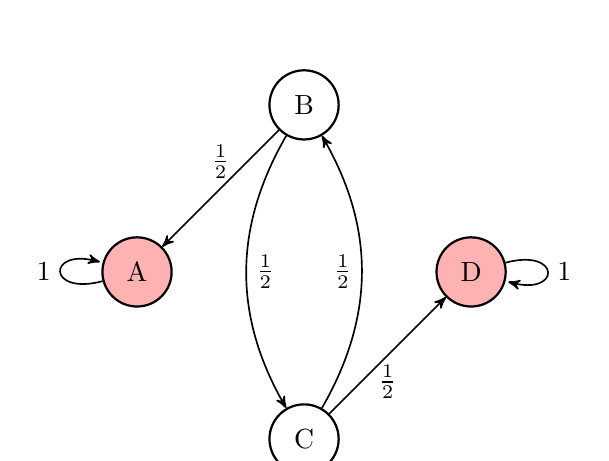
\begin{tikzpicture}[->,>=stealth',auto,semithick,node distance=3cm]
                \tikzstyle{every state}=[fill=white,draw=black,thick,text=black,scale=1]
                \node[state, fill=red!30]   (A)                     {A};
                \node[state]                (B)[above right of=A]   {B};
                \node[state]                (C)[below right of=A]   {C};
                \node[state, fill=red!30]   (D)[above right of=C]   {D};

                \path
                (A) edge[loop left]     node{$1$}               (A)
                (B) edge[above]         node{$\frac{1}{2}$}     (A)
                edge[bend right]        node{$\frac{1}{2}$}     (C)
                (C) edge[below]         node{$\frac{1}{2}$}     (D)
                edge[bend right]        node{$\frac{1}{2}$}     (B)
                (D) edge[loop right]    node{$1$}               (D);
            \end{tikzpicture}
        \end{center}
    }
    \task{Which states are absorbing states?}
    {

    }
    \task{$P^{(n)}_{i,j}$ denotes the probability that a player starts with $i$ coins and then ends up with $j$
        coins in $n$ steps. Show that for an even number steps $(n)$ for a game where no player
        wins/loses that $P^{(n)} = \rbra{\frac{1}{2}}^n $. Assume the same initial conditions given above.}
    {

    }
\end{enumerate}

\section{Mouse house}
A mouse is in a maze with four cells (1 -- 4) and a path to freedom (cell 0) that can only
be reached from cell 4. The transition matrix of the mouse in the maze is given below with
indices from 0 -- 4 on each axis.
\[
    P = \bordermatrix{
        & 0 & 1 & 2 & 3 & 4 \cr
        0 & 1 & 0 & 0 & 0 & 0 \cr
        1 & 0 & 0 & \frac{1}{2} & \frac{1}{2} & 0 \cr
        2 & 0 & \frac{1}{2} & 0 & 0 & \frac{1}{2} \cr
        3 & 0 & \frac{1}{2} & 0 & 0 & \frac{1}{2} \cr
        4 & \frac{1}{3} & 0 & \frac{1}{3} & \frac{1}{3} & 0
    }
\]

\begin{enumerate}
    \task{Draw the maze using the information from the transition matrix.}
    {
        \begin{center}
            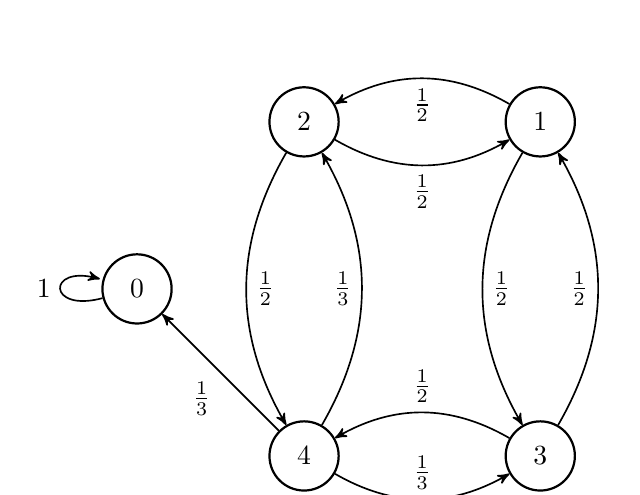
\begin{tikzpicture}[->,>=stealth',auto,semithick,node distance=3cm]
                \tikzstyle{every state}=[fill=white,draw=black,thick,text=black,scale=1]
                \node[state]    (A)                     {$0$};
                \node[state]    (C)[above right of=A]   {$2$};
                \node[state]    (B)[right of=C]         {$1$};
                \node[state]    (E)[below right of=A]   {$4$};
                \node[state]    (D)[right of=E]         {$3$};

                \path
                (A) edge[loop left]            node{$1$}               (A)
                (B) edge[bend right]           node{$\frac{1}{2}$}     (C)
                edge[bend right]               node{$\frac{1}{2}$}     (D)
                (C) edge[bend right, below]    node{$\frac{1}{2}$}     (B)
                edge[bend right]               node{$\frac{1}{2}$}     (E)
                (D) edge[bend right]           node{$\frac{1}{2}$}     (B)
                edge[bend right, above]        node{$\frac{1}{2}$}     (E)
                (E) edge[bend right]           node{$\frac{1}{3}$}     (C)
                edge[bend right]               node{$\frac{1}{3}$}     (D)
                edge                           node{$\frac{1}{3}$}     (A);
            \end{tikzpicture}
        \end{center}
    }
    \task{What is the probability that the mouse starts at 1 and then ends at 1 in two steps?}
    {

    }
    \task{What is the 2-step transition matrix?}
    {
        \[
            P^{(2)} = P^2 = \begin{pmatrix}
                1           & 0           & 0            & 0            & 0           \\
                0           & \frac{1}{2} & 0            & 0            & \frac{1}{2} \\
                \frac{1}{6} & 0           & \frac{5}{12} & \frac{5}{12} & 0           \\
                \frac{1}{6} & 0           & \frac{5}{12} & \frac{5}{12} & 0           \\
                \frac{1}{3} & \frac{1}{3} & 0            & 0            & \frac{1}{3} \\
            \end{pmatrix}
        \]
    }
\end{enumerate}

\section{Telephone calls}
The number of telephone calls arriving in a call center follows a Poisson process with a rate
of 1 phone call every 20 minutes $\rbra{\lambda = 3 \frac{1}{\text{hour}}}$.
What is the probability of getting at most
3 phone calls at time $[0, 1)$ (in hours), and then at least 4 phone calls at time $[1, 2)$, and
then at most 3 phone calls at time $[2, 3)$?

\section{Chapman-Kolmogorov}
A Markov chain has the transition probability matrix given below. What is the 2-step transition probability
$P^{(2)}_{0,2}$? Solve this problem two ways by using the Chapman-Kolmogorov
equation and by calculating the 2-step transition matrix.

\[
    P = \bordermatrix{
        & 0 & 1 & 2 \cr
        0 & 0.6 & 0.3 & 0.1  \cr
        1 & 0.2 & 0.5 & 0.3 \cr
        2 & 0.4 & 0.4 & 0.2
    }
\]

\section{Drunk friends}
Your three drunk friends (A, B, and C) are walking back home from a party in your
house. Because two of them (A and B) live together, you tie their hands together. One
hour later, you discover that none of them have reached their homes! Assume that each
person independently chooses to walk in a random direction (north, south, east, or west)
at a rate of 1 step per second, and that A and B will only move if they agree on the direction:
\begin{enumerate}
    \task{Simulate 500 possible trajectories of A (and B) and C after 1 hour.
        Plot the distributions of the distance from your house.}
    {

    }
    \task{From the results of your simulation, how far away from your house should you search
        for A (and B) and C to have a 60\% chance of finding each of them?}
    {

    }
\end{enumerate}

\end{document}